\section{Teilaufgabe 4}
\begin{aufgabe}
    Zeichnen das asymptotische Bode-Diagramm vom $P_1(s)$ im angehängten 
    leeren Bodediagramm.
\end{aufgabe}
\begin{figure}[h!]
    \centering
    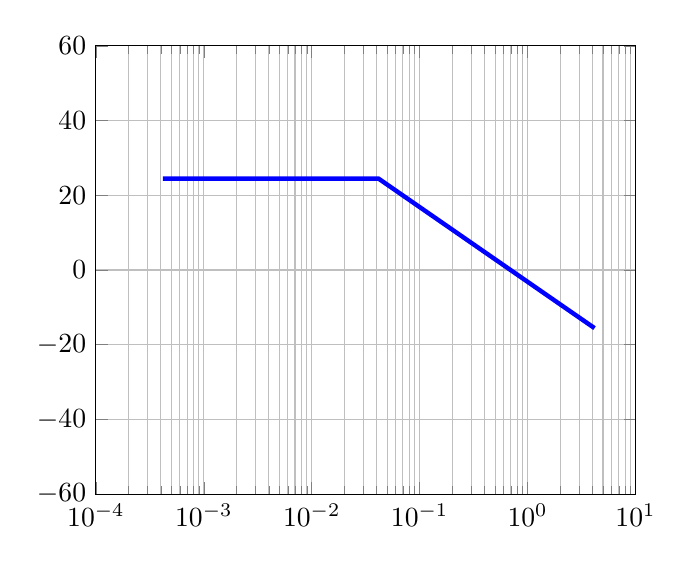
\begin{tikzpicture}
        \begin{semilogxaxis}
            [xmin=1e-4, 
                xmax=1e1, 
                ymin=-60, 
                ymax=60, 
                ytick={-60, -40, ..., 60}, 
                grid=both]
            \addplot[mark=none, color=blue, ultra thick] coordinates 
                {(0.000417,24.430) 
                (0.0417,24.430) 
                (4.17,-15.57)};
        \end{semilogxaxis}
    \end{tikzpicture}
    \\
    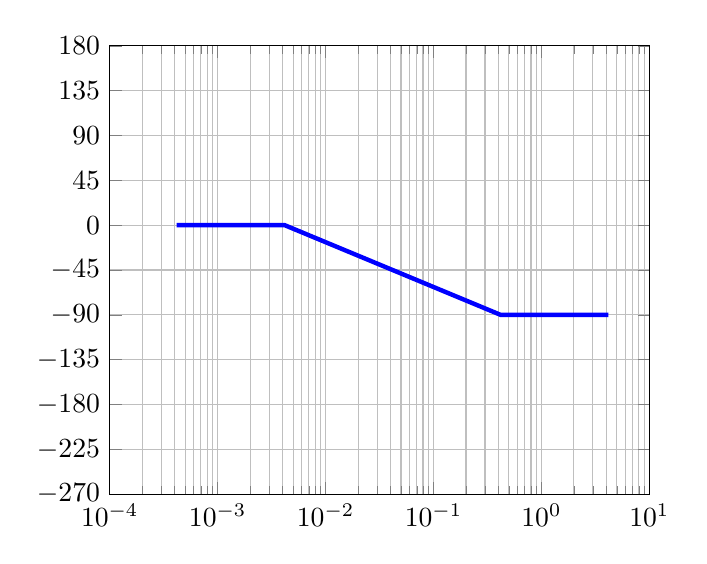
\begin{tikzpicture}
        \begin{semilogxaxis}
            [xmin=1e-4, 
                xmax=1e1, 
                ymin=-270, 
                ymax=180, 
                ytick={-270, -225, ..., 180}, 
                grid=both]
            \addplot[mark=none, color=blue, ultra thick] coordinates 
                {(0.000417,0) 
                (0.00417,0) 
                (0.417,-90) 
                (4.17,-90)};
        \end{semilogxaxis}
    \end{tikzpicture}
\end{figure}
